Wenn eine Anwendung entwickelt werden soll, ist die Wahl des richtigen Frameworks oder auch der Programmiersprache eine wichtige Entscheidung für das Projekt. Viele Entscheidungen können im Verlauf der Entwicklung noch abgeändert werden, aber um eine derartige Entscheidung zu ändern, müssen Teile der Anwendung oder auch der komplette Quellcode neu geschrieben werden. Neben Unsicherheiten bei der richtigen Wahl erscheinen täglich neue Artikel, die über neue Standards in der Appentwicklung informieren wollen. So ist eine derartig wichtige Entscheidung oft sehr schwierig.

Da Anwendungen meistens nicht nur auf einem Gerätetyp, sondern allen Nutzern auf den verschiedensten Plattformen zur Verfügung stehen sollen, hat diese Entscheidung noch einmal eine größere Bedeutung, da sie eng verbunden mit den Kosten der Entwicklung und dem Nutzungserlebnis ist.

In Zeiten der Heimcomputer und des stetig wachsenden Internets war der einfachste Weg, eine Webseite zu entwickeln, die über den Browser der genutzten Geräte aufgerufen werden konnte. Mit der Ära der Smartphones jedoch änderte sich das. So waren Webapplikationen oft nicht für die Nutzung an derartig kleinen Geräten mit einer Toucheingabe angepasst.

Die Nutzung von Smartphones öffnete außerdem die Tür, andere Funktionalitäten, wie die Kamera, Bluetooth oder GPS-Daten zu nutzen. Deshalb wurden Applikationen oft nativ mit Objectiv-C, beziehungsweise Swift, für iOS und Java, mittlerweile Kotlin, für Android entwickelt. Durch die Programmierung mit Hilfe der nativen Programmiersprachen, entstehen optimal für die einzelnen Plattformen angepasste Anwendungen.

Durch den Wunsch nach einer Multi-Plattform Anwendung jedoch, also einer App, die für mehrere Plattformen veröffentlicht werden soll, muss bei der nativen Entwicklung für jede Plattform eine eigene Applikationen in der jeweiligen Programmiersprache und Technologie geschrieben werden. Dadurch entsteht ein hoher Aufwand und die Kosten multiplizieren sich mit der Zahl der abzudeckenden Plattform.

Deswegen wurden bereits früh sogenannten Cross-Plattform Technologien entwickelt, die es ermöglichen, mit einem geteilten Code so viele Plattformen wie möglich abzudecken. So erschien etwa 2008 PhoneGap. Es war ein Open-Source Framework zur Entwicklung von hybriden mobilen Applikationen, die mit Hilfe von HTML, CSS und JavaScript programmiert wurden. PhoneGap und sein Nachfolger Cordova waren einige Zeit auch sehr beliebt in diesem Bereich, 2019 hatten beide zusammen immerhin einen Marktanteil von etwa 40\% unter den Cross-Plattform Frameworks \cite{statist_CP_Framework}.

Trotz der verringerten Kosten werden dennoch viele Applikationen immer noch nativ entwickelt. So ergab eine interne Untersuchung der Firma ScanBot SDK\footnote{https://scanbot.io/de/blog/native-apps-vs-cross-platform/}, dass 2019, 57\% ihrer Nutzer native Applikationen entwickelten, obwohl ihr Produkt ebenso für viele der gängigen Cross-Plattform Frameworks zur Verfügung steht.

Ein Grund für Unsicherheit in diesem Bereich sind oft auch negative Erfahrungsberichte von Firmen, die einen Umstieg von nativ zu Cross-Plattform-Applikationen versuchten.  So etwa auch Airbnb \cite{Airbnb_react_goals}. Sie nutzten das von Facebook mitentwickelte Framework React Native. 2019 hatte dieses Framework einen Marktanteil von 42\% \cite{statist_CP_Framework}. 

Ihre Ziele waren einfach:
\begin{enumerate}%This could be compactenum or inparaenum see paralist dokumentation%
    \item Schnelleres entwickeln.
    \item Die gleiche Codequalität beibehalten.
    \item Nur noch eine Codebasis.
    \item Die Entwicklungsabläufe verbessern.
\end{enumerate}
%%\nointerlineskip
Jedoch traten während der Entwicklung einige technische Probleme auf. So mussten etwa eine eigene Version des genutzten Frameworks erstellt werden, um notwendige Änderungen einzubauen. Dies erschwerte es jedoch Updates des Frameworks zu integrieren \cite{Airbnb_technology}. Die Entwickler von Airbnb erkannten deshalb, dass sie ihre Ziele nicht einhalten konnten und kehrten 2018 wieder zu einem nativen Ansatz zurück.

Durch Beispiele wie dieses, sind App-Entwickler oft skeptisch gegenüber derartigen Lösungen, da dies auch immer mit großen Änderungen, hohen Investitionen und einer  Einarbeitungszeit verbunden sind \cite{medium_Lehtimäki}. Dennoch nimmt die Zahl der Cross-Plattform Entwicklungen in den letzten Jahren zu. So ergab die Untersuchung von ScanBot SDK, dass 2021, gerade einmal zwei Jahre später, 58\% Cross-Plattform Lösungen nutzten, also ganze 15\% mehr. Diese Zahl stützt auch eine Untersuchung von Jetbrains \cite{JetBrains_miscellaneous_2021}. Diese ergab, dass 2021 53\% aller App Entwickler, derartige Technologien nutzten .

\begin{figure}[ht]
  \centering
  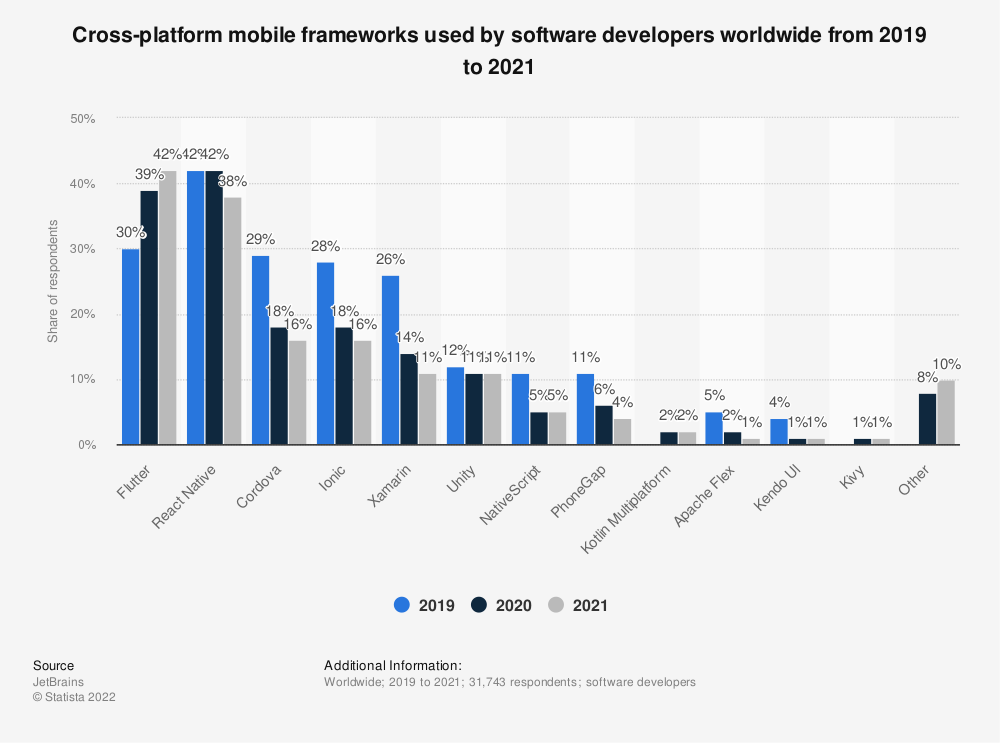
\includegraphics[width=15cm,keepaspectratio]{images/cross-platform-mobile-frameworks.png} 
  \caption[Statistik Cross-Plattform-Frameworks]{Cross-Plattform-Frameworks 2019-2021 \cite{statist_CP_Framework}}
  \label{fig:statista_cross_plattform}
\end{figure}

Diese Zahl dürfte in den nächsten Jahren weiter steigen. Einen Grund dafür bieten unter anderem auch neue Frameworks die entstehen. In Abbildung \ref{fig:statista_cross_plattform} ist eine Statistik zu sehen, die die Verteilung von verschiedenen Cross-Plattform-Entwicklungstechnologien zwischen 2019 und 2021 zeigt. Sie zeigt wie schnell sich die Verteilung von Cross-Platform Frameworks ändern kann. Flutter ist dafür ein gutes Beispiel. Es ist ein Framework das erst 2017 auf den Markt gekommen ist und innerhalb von gerade einmal 4 Jahren auf einen Marktanteil von 42\% gekommen ist. Von einigen wird es als der neue Standard angesehen und einige Unternehmen steigen auf Flutter um. 

Jedoch gibt es auch Entwickler, die weiterhin nativ entwickeln. So etwa die Appagentur Number42, mit der diese Arbeit in Zusammenarbeit entstanden ist. Sie entwickeln Web und mobile Applikationen. Alle der dort entwickelten mobilen Applikationen sind mit den nativen Programmiersprachen geschrieben. Einerseits entwickeln sich auch die nativen Programmiersprachen stetig weiter und erhalten Änderungen, die eine Entwicklung vereinfachen und beschleunigen. Andererseits gibt es auch Projekte, bei denen lediglich eine Plattform benötigt wird, da sie nur auf Geräten des Unternehmens ausgeführt werden sollen und diese beispielsweise nur Smartphones der Firma Apple nutzen. Deswegen ist auch dieser Ansatz nicht von der Hand zu weisen und es kann durchaus sinnvoll sein, neue Apps weiterhin nativ zu entwickeln.

\section{Beitrag dieser Arbeit}
Der primäre Inhalt dieser Arbeit ist die Beschreibung vier verschiedener Implementierungen und deren Vergleich anhand verschiedener Kriterien. Dafür werden Daten aus der Implementierung, Dokumentationen und anderen Quellen gesammelt und verglichen.
Um ein einheitliches Verständnis für die verschiedenen Applikationsklassen zu erhalten, werden diese zunächst vorgestellt und etwas erklärt, da es viele verschiedene Einordnungen und Klassifizierungen in wissenschaftlichen Papieren gibt.
Dabei wird eine native Android Applikation mit Kotlin, eine hybride Applikation mit Kotlin, eine Cross-kompilierte Applikation mit Flutter und eine gemischte Implementierung aus einer Cross-kompilierten und einer hybriden Applikation mit Flutter vorgestellt. 
Dabei sollen auf die Kriterien Performance und Entwicklung, Entwicklergemeinschaft, Entwicklungsdauer, Benutzeroberfläche(UI) und Funktionalität eingegangen werden. Dabei soll analysiert werden welche Implementierung in welchen Kriterien besser abschneidet und eine Erklärung und Einordnung geschehen, um eine Wahl des passenden Ansatzes zur Entwicklung einer Multi-Plattform-Anwendung zu erleichtern.


\section{Aufbau der Arbeit}
In Kapitel 2 werden zunächst verwandte Arbeiten vorgestellt, während in Kapitel 3 die verschiedenen Applikationsklassen, einige Begriffe und die Implementierungen vorgestellt und die Arbeit abgegrenzt.
Danach werden in Kapitel 4 die verschiedenen Implementierungen und einige Erkenntnisse während der Entwicklung erklärt. Dabei soll auch auf Stärken und Schwächen der einzelnen Implementierungen eingegangen werden, die während der Implementierung und Recherche aufgefallen sind.
In Kapitel 5 soll anschließend eine Auswertung der Implementierungen anhand einiger Kriterien stattfinden und mit weiteren Erklärungen und Vergleichen, eine Einordnung der verschiedenen Ansätze stattfinden. Abschließend soll in Kapitel 6 ein Fazit gezogen werden und ein Ausblick auf künftige Arbeiten gegeben werden.